\documentclass{ucph-handout}
%\usepackage[english]{babel}
\usepackage{hyperref}

\usepackage{wrapfig}
\newcounter{handout}
\newcommand{\Ark}{Worksheet \arabic{handout}: }
\renewcommand{\Title}{\Ark Kickstart Day 2 Special}%
\renewcommand{\TimeAndLocation}{DIKU, 2023}%
\renewcommand{\Author}{Daniel Spikol}
\renewcommand{\AuthorEmail}{ds@di.ku.dk}

\begin{document}

%==WORKSHEET 2 
\newpage
\stepcounter{handout}

\begin{exercisebox}[adjusted title = Mouse input and Functions]
Functions make it possible to reuse the same code in several places,
name entire blocks of code and structure code.\\

In this alternative worksheet, you get break from the Fishes and the Green City and to work with the Cyclops to explore mouse Input and the Environment.

\noindent
Open a new project and name it ``cyclops\_mouse''. BEMÆRK! NOTE! Line indentation with 4 spaces is important!

\tcbsubtitle{Exercise:} 
Type in this code to make the basis for the cyclops. The exercise aims to for you update the code to:
\begin{enumerate}
\item Have the Cyclops follow the mouse around the in the  \ttpy{def draw()} function
\item Draw the mouth into the \ttpy{def draw_cyclops(x, y)}
\end{enumerate}


\begin{python}
# Cyclops properties
cyclops_x =200
cyclops_y = 200
cyclops_radius = 50

def setup():
    size(800, 600)
    background(255)

def draw():
    background(255)  # Clear the screen each frame

    # Update cyclops position to follow the mouse
    # This is where you put your code in...

    # Draw the cyclops
    draw_cyclops(cyclops_x, cyclops_y)
\end{python}

Now add the \ttpy{def draw_cyclops(x, y)} function
\begin{python}
def draw_cyclops(x, y):
    # Head of the cyclops
    fill(200, 200, 250)
    ellipse(x, y, 2 * cyclops_radius, 2 * cyclops_radius)

    # Eye of the cyclops
    fill(255)
    ellipse(x, y-10, cyclops_radius, cyclops_radius)
    
    # Pupil of the cyclops
    fill(0)
    ellipse(x, y-10, cyclops_radius / 4, cyclops_radius / 4)
    
    # Mouth of the cyclops
    # This is where you put your code in...
    
    
\end{python}
\end{exercisebox}

\newpage

\begin{exercisebox}[adjusted title= Extras]
\begin{itemize}
\item You want to be sure to add the mouth to the Cyclops
\item Also to make it move with your mouse
\item Maybe you make it smile or some other emotions...
\end{itemize}

\begin{minipage}{0.60\linewidth}
Investigate the  built-in  \ttpy{mouseX} functions and the other functions in the \href{https://py.processing.org/reference/}{Py.Processing Reference}  
\end{minipage}

\begin{minipage}{0.40\linewidth}
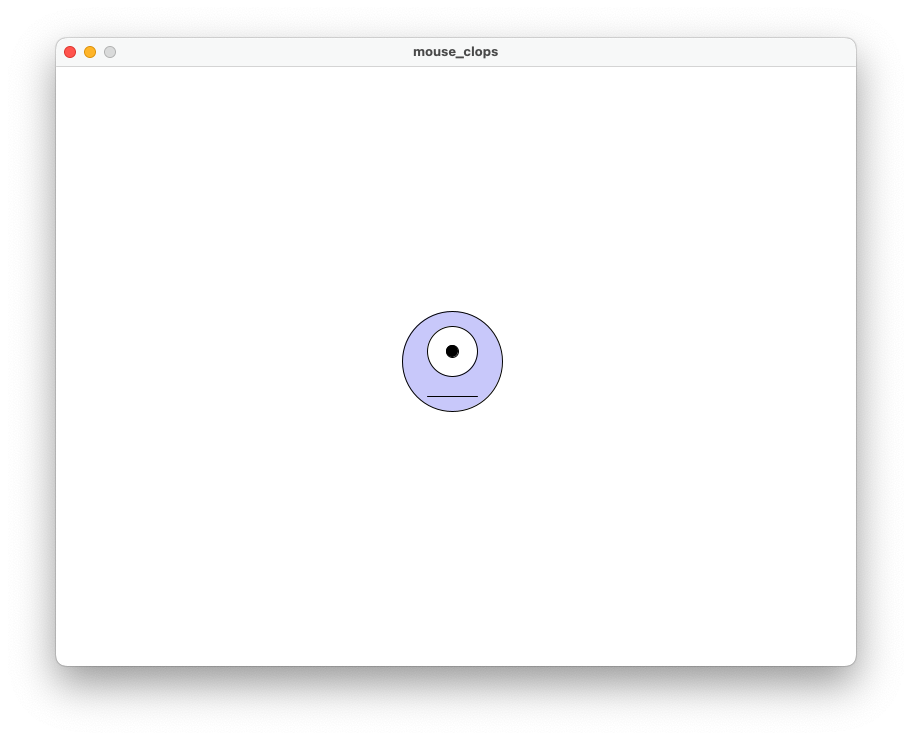
\includegraphics[width=2.5\textwidth]{illustrationer/cyclops_mouse} 
\end{minipage}
~
\end{exercisebox}


\end{document}